\documentclass{article}
\usepackage[utf8]{inputenc}
\title{Lecture 3: controlling Complexity: Feature Selection and Regularization}
\author{wbg231 }
\date{December 2022}
\newcommand{\R}{$\mathbb{R}$}
\newcommand{\B}{$\beta$}
\newcommand{\A}{$\alpha$}
\newcommand{\D}{\Delta}

\newcommand{\avector}[2]{(#1_2,\ldots,#1_{#2})}
\newcommand{\makedef}[2]{$\textbf{#1}$:#2 }
\usepackage{tikz,graphicx,hyperref,amsmath,amsfonts,amscd,amssymb,bm,cite,epsfig,epsf,url}

\begin{document}

\maketitle

\section*{introduction}
\begin{itemize}
\item \href{https://nyu-ds1003.github.io/mlcourse/2023/lectures/lec03/03-handout.pdf}{lecture slides}
\section{model complexity}
\subsection{complexity of the hypothesis space}
\item approximation error (of \mathcal{F}) $R(f_{\mathcal{F}})-R(f^{*})$ ie the distance between the over all best function and the best function within our hypothesis space
\item Estimation error of ($\hat{f}_{n} \in \mathcal{F})$ $R(\hat{f}_{n}-R(f_{\mathcal{F}})$ ie the distance between the best function possible in the hypothesis space and the best function we are able to find with the given data
\item what is the trade off between approximation error and estimation error 
\begin{itemize}
    \item bigger $\mathcal{F}$ means we have a better approximation but can lead to over fitting so that is lower approximation error but higher estimation error 
    \item smaller $\mathcal{F}$ less likely to over fit but the best function within the space may be further from the optimal function, so lower estimation error higher approximation error
\end{itemize}
\item so we want to find a middle ground for the size of $\mathcal{F}$
\item to do that we need some measure of the complexity of $\mathcal{F}$
\item some measures could be the number of variables we are modeling or the number of features, or something like the degree of the polynomial we are using to fit. 
\subsection{General approach to control complexity}
\item step 1. learn a sequence of models varying in complexity on the training data $$\mathcal{F}_1\subset ... \subset \mathcal{F}t$$
\item so in the case of the polynomial functions $\mathcal{F}=\{$ all polynomial functions $\}$ and $\mathcal{F}_d=\{$ all polynomial functions of degree $\leq d\}$ 
\item step 2. select one of these models based on a score (for instance validation error)
\subsection{example}
 \item so for feature selection in linear regression a nested sequence of hypothesis space could be $$\mathcal{F}_1\subset ... \subset \mathcal{F}t$$
 \item where $\mathcal{F}=\{$ linear functions using all features $\}$
 \item where $\mathcal{F}_{d}=\{$ linear functions using less than d features $\}$
\item if this were the case the problem becomes about choosing an optimal subset 
\begin{itemize}
    \item that is choosing the subset of features that is best according to our scoring function. so for instance, in a model with train models using $\{\},\{X_1\},\{X_2\},\{X_1,X_2\}$ respectively and see which has the best score
    \item this is not an effluent algorithm iterating over all subsets become very expensive with a large number of features this is a $O(2^n)$ algorithm  
\end{itemize}
\subsection{greedy subset selection}
\item we could more efficiently find the optimal subset using greedy algorithms 
\item one such approach is forward selection
\begin{enumerate}
    \item start with an empty set of features S
    \item for each feature i not in S
    \begin{itemize}
        \item learn a model using features $S\cup i$
        \item compute the score of the model $\alpha_i$
    \end{itemize}
    \item find the candidate feature with the highest score j=$argmax \alpha_i$
    \item if $\alpha_i$ improves the current best score then add the feature j that is $S\leftarrow S\cup j$ and go back to the start of the loop. otherwise return S
\end{enumerate}
\item we can also do backwards selection, which is more or less the same algorithm except we start with S as all features then remove the worse feature until removing the worst feature no longer increases our score
\subsection{feature selection: discussion}
\item in general think of the number of features as a measure of model complexity of a linear function 
\item general approach to feature selection 
\begin{itemize}
    \item define a score function that balances the training error and complexity
    \item find the subset of features that minimizes the score
\end{itemize}
\item forward and backward do not guarantee the best overall subset 
\item also forward and backward selection do not guarantee they will return the same result, they could return local optimums

\section{regularization}
\subsection{complexity penalty}
\item a score should balance the training loss and some measure of complexity an example score function could be $$score(S)=training_loss(S)+\lambda|S|$$ $\lambda \in \mathbb{R}$ balances the training loss and the number of features in the model (which is a measure of complexity)
\begin{itemize}
    \item adding an extra feature must be justified by at least $\lambda$ improving in the training loss
    \item larger $\lambda$ means that complex models are penalized more heavily
\end{itemize}
\item the goal of a score function is to balance the complexity of the hypothesis space $\mathcal{F}$ and the training loss
\item a complexity measure is a function $\Omega: \mathcal{F}\rightarrow [0, \infty)$ that is which maps the hypothesis space to some real number. for instance the number of features
\item we define Penalized empirical risk minimization or Tikhonov regularization for a complexity measure $\Omega: \mathcal{F}\rightarrow [0, \infty)$ and $\lambda \geq 0$ as $$min_{f\in \mathcal{F}}\frac{1}{n}\Sigma_{i=1}^{n}\ell(f(x_i),y_i)+\lambda \Omega(f)$$
\item the number of features as a complexity measure is very hard to optimize because it is non-continuous value 
\item so we are going to want to define some function that will allow us to optimize both terms at once 
\subsection{weight shrinkage: intuition}

    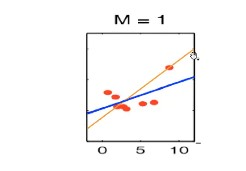
\includegraphics[width =10cm]{lecture_notes/lecture_3/immages/l3_1.jpg}
    \item suppose we are training a linear function to fit your data (the read dots in the above image)
    \item and suppose we fit two linear models to this data the yellow and blue lines that each have the same training loss
    \item which model to we prefer? the blue because it has a lower slope
    \item we always like a smaller slope unless the data supports it which in this case it does not since both the blue and orange lines have the same training error
    \item when we have a larger slope the output is very sensitive to small changes in the training data
    \item also can see the Orange line is very impacted by the upper most red line so if we removed it we would get a very different orange line 
    \item having larger weight ts  makes our model less robust to outliers, so a smaller slope means the model is less sensitive to noise in the data
\subsection{weight shrinkage regression}
    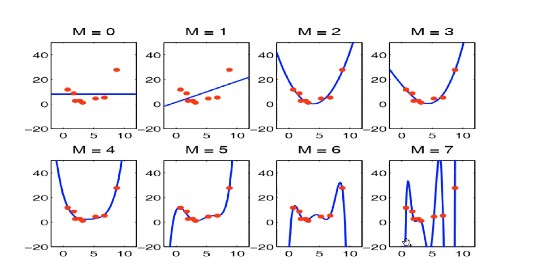
\includegraphics[width =10cm]{lecture_notes/lecture_3/immages/l3_2.jpg}
\item we are trying to fit the red dots with different degrees of models 
\item the quadratic curve seems to fit the model really well, but we can get a better fit, by raining the degree of the polynomial higher and higher
\item  but the higher degree polynomial wiggles a lot it is very sensitive to input data
\item the larger the weights on higher order terms the less robust our models will be to input data
\item so we want to keep the magnitude of the weights that we put in each term of the model as small as possible
\subsection{linear regression }
\item we have a linear model with hypothesis space $$\mathcal{F}=\{f:\mathbb{R}^{d}\rightarrow \mathbb{R} | f(x)=w^{T}x for w\in \mathbb{R}^{d} \}$$ ie the set of linear models mapping from the dimension of the input data to real numbers
\item assume we are using square loss so that is $\ell(\hat{y},y)=(y-\hat{y})^{2}$
\item and we have training data $\mathcal{D}_{n}=((x_1,y_1)..(x_n,y_n))$
\item the linear least squared ERM for square loss is $$\hat{W}=\argmin_{w\in \mathb{R}^{d}}\frac{1}{n}\Sigma_{i=1}^{n}(w^tx_i-y_i)^2$$
\item this model often over fits when the dimension of the data is much larger than n the number of samples 
\subsection{linear regression with l2 regularization}
\item we can try to avoid this over fitting using linear regression with l2 regularization ie ridge regression $$\hat{W}=\argmin_{w\in \mathb{R}^{d}}\frac{1}{n}\Sigma_{i=1}^{n}(w^tx_i-y_i)^2+\lambda||2||_{2}^{2}$$
\item this adds a term that penalizes the magnitude of weights
\item if $\lambda=0$ then this is just least squares regression 
\item $l_2$ regularization can be applied to any type of model by just adding $\lambda||w||_{2}^{2}$ to your objective function 
\subsection{l2 regularization reduces sensitivity to changes in input}
\item $\hat{f}(x)=\hat{w}^{t}x$ is lipshitz continuous with constant $L=||\hat{w}||_{2}$
\item this means that when moving from x to x+h $\hat{f}(x)$ changes no more than $L|h|=||\hat{w}||_{2}|h|$
\item so in other words, if our input data changes by a small amount due to noise then we can bound how much our resulting model will change
\item $\ell_{2}$ regularization controls the rate of change of the best model we taring on our data $\hat{f}(x)$
\item proof
\begin{itemize}
\item $|\hat{f}(x+h)-\hat{f}(x)|=|\hat{w}^{t}(x+h)-\hat{w}x|=|\hat{w}^{t}h\leq ||w|| ||h||$ by Cauchy Schwartz inequality
\end{itemize}
\item there are other norms that we can use to bound L 
\subsection{OLS regression vs ridge regression}
\item objective
\begin{itemize}
    \item OLS : $L(w)=\frac{1}{2}||Xw-y||_{2}^{2}$
    \item ridge $L(w)=\frac{1}{2}||Xw-y||_{2}^{2}+\frac{\lambda }{2}||W||_{2}^{2}$
\end{itemize}
\item gradient 
\begin{itemize}
    \item OLS $\nabla L(w)=X^{t}(Xw-y)$
    \item Ridge: $\nabla L(w)=X^{t}(Xw-y)+\lambda w$
    \item so we have this added term to our gradient $\lambda w$ in neural nets this is often called weight decay
\end{itemize}
\item both have closed form solutions
\begin{itemize}
    \item OSL: $X^{t}xw=X^{t}y$
    \item Ridge: $(X^{T}X+\lambda I)w=X^{t}y$ ridge regression  is a bit nicer because $(X^{t}X+\lambda I)$ is always invertable \href{https://math.stackexchange.com/questions/1647625/when-is-mathbfxt-mathbfx-lambda-mathbfi-invertible}{due to this}
\end{itemize}
\subsection{Rodger regression regularization path path}
\item $\hat{w}_{w}=armin_{||w||^{2}_{2}\leq r}\frac{1}{n}\Sigma_{i=1}^{n}(w^{t}x_i-y_i)^2$ that is the weights leaned With the constraint such that the sum of the squared weights is less than a constant $r^2$
\item $\hat{w}=\hat{w}_{\infty}$ that is unconstrained Empirical risk management 
\item for r=0 $\frac{||\hat{w}_{r}||_{2}}{||\hat{w}||_{2}}=0$ basically that is we have constrained our optimization so much in the rusticated case such no weights are learned 
\item if $r=\infty$ then $\frac{||\hat{w}_{r}||_{2}}{||\hat{w}||_{2}}=1$ that is we are not constraining our weights at all so the ratio of the weights with this constraint and no constraint is 1. 
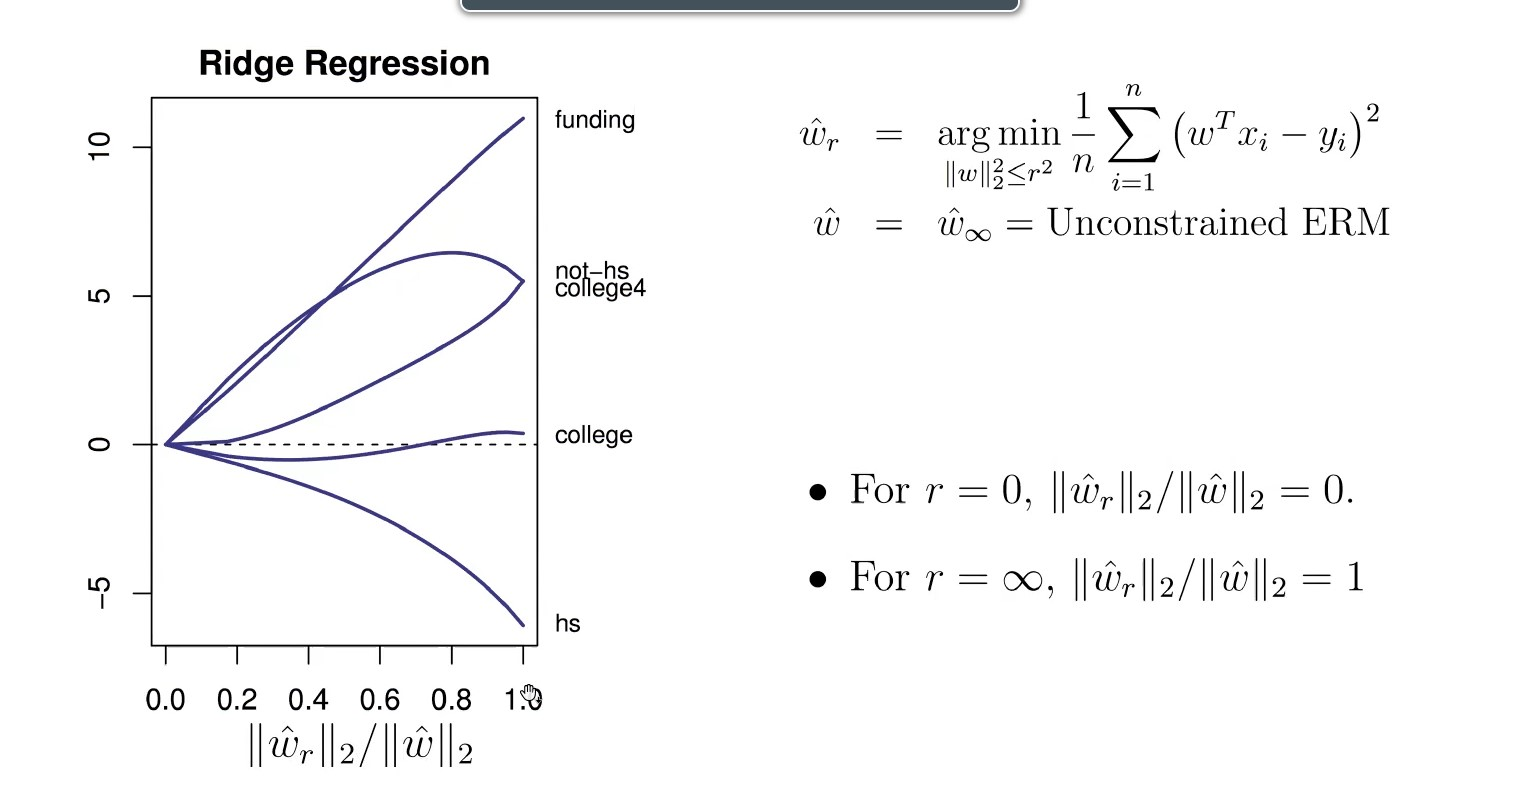
\includegraphics[width=10cm]{lecture_notes/lecture_3/immages/l3_3.jpg}
\item so the y axis is the ratio of regularized weights over unconstrained weights 
\item at the right side of the graph there is no constraint ie $\lambda=0$
\item the y axis is the magnitude of the regulated weights. so note that to the right the magnitude of the weights are going down as we increase $\lamnda$ 

\subsection{lasso regression}
\item instead of applying $\ell_2$  we can use $\ell_{1}$ norms 
\item lasso regression sues this $\ell_{1}$ norm 
\item lass regression also called tikhonovs form is $$\hat{w}=armin_{w\in \mathbb{R}^{d}}\frac{1}{n}(w^{t}x_{i}-y_{i})^2+\lambad ||w||_{1}$$
where $||w||_{1}=\Sigma_{i=1}^{d}|w_i|$

\subsection{ridge vs lassos regularization paths}
\item 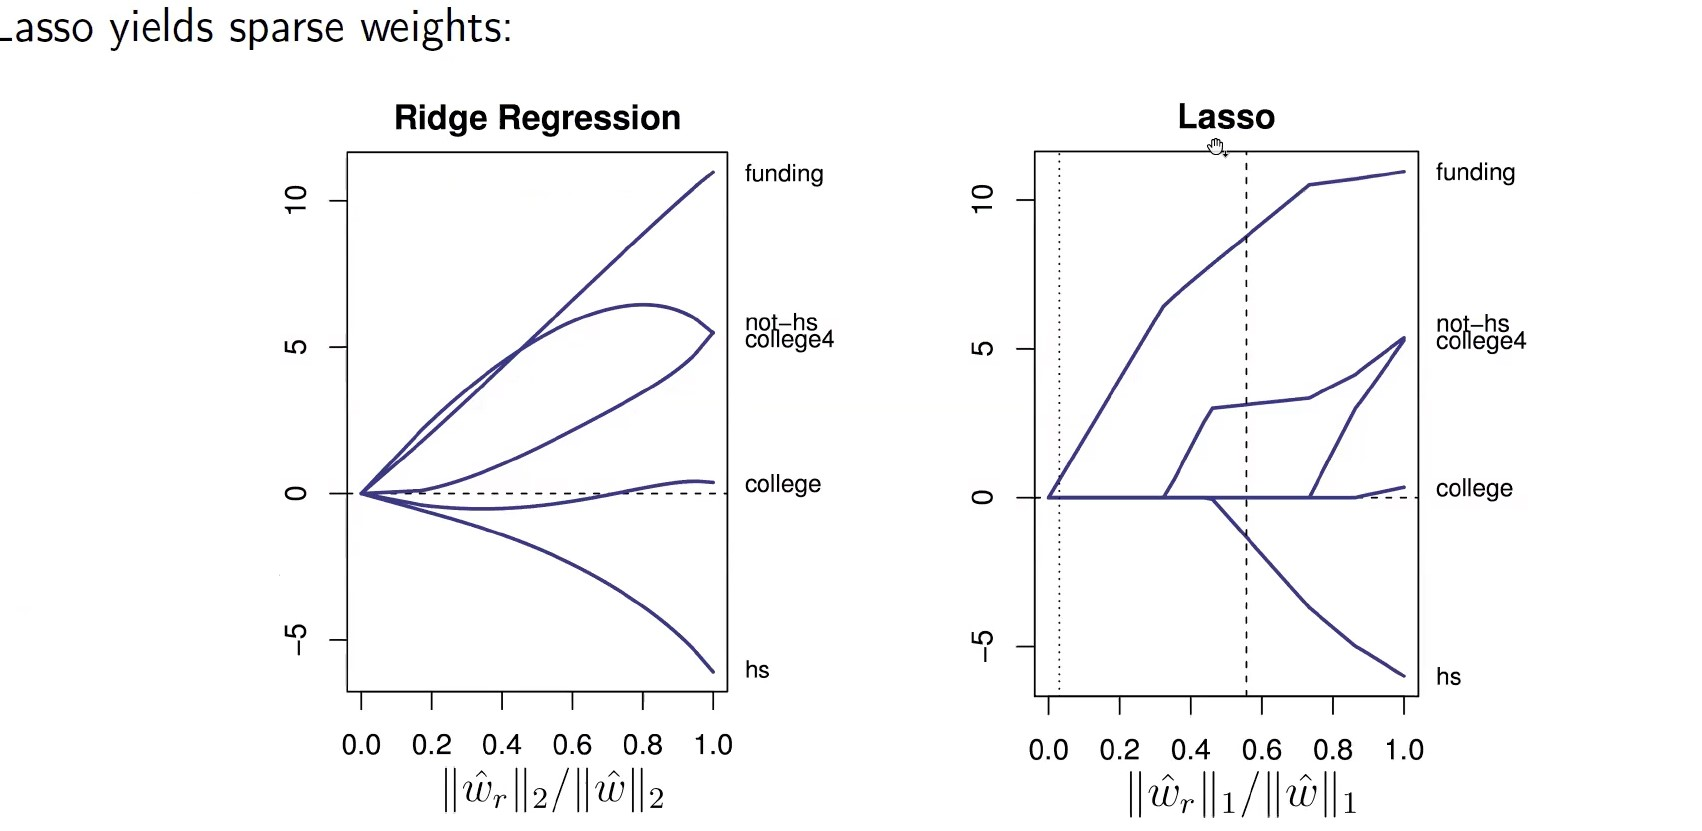
\includegraphics[width=10cm]{lecture_notes/lecture_3/immages/l3_4.jpg}
\item lasso
\begin{itemize}
\item lasso regression is almost piece wise linear, that is at different stages the weights are decreasing by a linear amount 
\item further in lasso regression the coefficients of some features will shrink directly to zero, before we have a very large $\lambda$
\item we are more liekly to observe weights that are zero. 
\end{itemize}
\item in ridge regression 
\begin{itemize}
    \item everything converges to zero at the very end.
    \item also wights do not decrease in a linear way 
\end{itemize}


\subsection{the benefits of sparsity}
\item why is sparsity good? 
\item if the coefficient for a parameter is zero Thant means the feature is not needed for prediction. meaning 
\begin{itemize}
    \item faster to compute features, ie we need to use less features in our computation 
    \item we need to store less features in the memory, if we know there parameter is zero
    \item having zero in your weights improves intractability because it makes it easy to identify important features by looking at non zero weights
    \item prediction function may also generalize better, because the model is less complex because it uses less feature dimensions 
\end{itemize}
\section{why does l1 regularization lead to sparsity?}
\subsection{regularization as constraint empirical risk minimization}
\item constraint ERM or (Ivanov regularizing ) for a complexity measure $\Omega:\mathcal{F}\rightarrow[0,\infty]$ and fixed $r\geq 0$ $$min_{f\in \mathcal{F}}\frac{1}{n}\ell(f(x_i),y_i) \\\quad \text{ s.t. } \Omega(f)\leq r$$
\item here the regularization is in the constraint of the function
\item we can write lasso regression as constrained erm as$$\hat{w}=argmin_{||w||_{1}\leq r}\frac{1}{n}(w^{t}x_i-y_i)^2$$
\item here $r$ and $\lambda$ have the same function 
\subsection{ivanov vs tikhnon regularization}
\item tikhnon regularization or penalized erm is $$min_{f\in \mathcal{F}}\frac{1}{n}\Sigma_{i=1}^{n}\ell(f(x_i),y_i)+\lambda\Omega(f)$$ 
\item ivanov or constrained erm is $$min_{f\in \mathcal{F}}\frac{1}{n}\ell(f(x_i),y_i) \\\quad \text{ s.t. } \Omega(f)\leq r$$
\item consider $L:\mathcal{F}\rightarrow R$ be any performance measure of f 
\item for many $L, \Omega$ constrained and penalized ERM are the same. that is is any optimal we obtained with penalized erm we can get with constrained erm and vice versa
\item that comes from Lagrangian duality theory
\item in practice we will use which ever is more use full 


\subsection{l1 and l2 norm constraints}
\item lets consider $\mathcal{F}=\{w_1x_1+w_2x_2\}$ ie two dimensional problem  
\item we can represent each function in $\mathcal{F}$ as a point $(w_1,w_2)\in\mathbb{R}^{2}$
\item where in $\mathcal{R}^{2}$ are the functions that satisfy the constrained erm for $\ell_1$ and $\ell_{2}$
\item 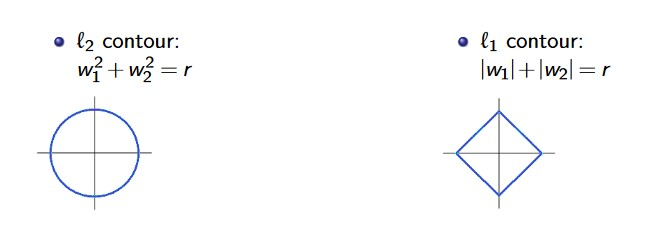
\includegraphics[width=10cm]{lecture_notes/lecture_3/immages/l3_5.jpg}
\item these are contour lines for the different norms 
\item that is we can see that all points on the right circle $(w_1,w_2)$ will have $||w||_{2}=w_1^2+w_2^2=r$ so we will select only points on the radius r
\item the $l_1$ contour is more like a diamond. that means $|w_1|+|w_2|=r$
\item so for constrained erm we can only select points within these two contours $l_2,l_1$
\item where on this plot are the spare solutions? that is where does either $w_1$ or $w_2$ equal zero? an the axis. so the x axis, y axis or origin. so there are 5 places we can get a spare solution in both cases.. 
\subsection{visualizing l2 regularization}
\item suppose we are looking at the constrained erm problem with $\ell_{2}$ penalties that is $f^{*}=argmin_{w\in \mathbb{R}^{2}} \Sigma_{i=1}^{n}(w^{t}x_i-y_i)^{2}\text{ such that } w_1^2+w_2^2\leq r$ 
\item 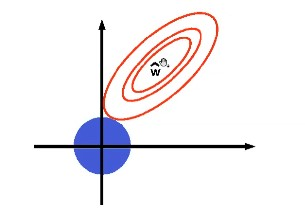
\includegraphics[width=10cm]{lecture_notes/lecture_3/immages/l3_6.jpg}
\item so in this plot the red lines are contours of our objective (training loss) function 
\item while the blue Circe is the region such that our constraint is satisfied in other words $w_1+w_2\leq r$
\item so $\hat{w}$ is the min of our training loss,that is the unconstrained optimal then the ellipses out form it increase training loss a little bit each time 
\item so we want the highest value of our taring loss (red function) within the bounds of the blue region (our constraint). 
\item thus we would chose the point on the very outside of our blue Circe and that point of intersection is our optimal
\item geometric intuition 
\begin{itemize}
    \item if we are projecting our solution onto a cirle region we will project onto the nearest neightbor. 
    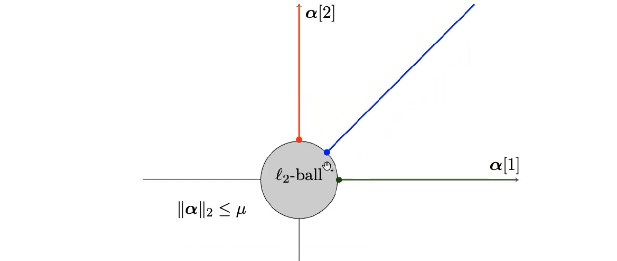
\includegraphics[width=10cm]{lecture_notes/lecture_3/immages/l3_9.jpg}
    \item we can see that the closest neighbor is only the corner if you are already on the axis, so it is much less liekly to get a conrener sollution 
    \item so if we are not on the corner already we will not og ot one 
    \item so this means that $\ell_{2}$ regualization priorties all directions equality
\end{itemize}

\subsection{visualizing l1}
\item suppose we are instead looking at $\ell_{1}$ constrained erm $f^{*}=argmin_{w\in \mathbb{R}^{2}} \Sigma_{i=1}^{n}(w^{t}x_i-y_i)^{2}\text{ such that } |w_1|+|w_2|\leq r$ 
\item 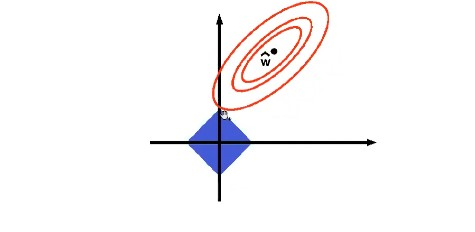
\includegraphics[width=10cm]{lecture_notes/lecture_3/immages/l3_7.jpg}
\item so where our objective function (training loss) and constraint would intersect in this case is on the axis, meaning that our found solution would be sparse. 
\item that is in this case we would learn a function on the y axis meaning $w_1=0$ would be true 
\item this is because the $\ell_{!}$ circle has four corners and it is much more easier to git the corner than not hit the corner 
\item geometric intuition 
\begin{itemize}
    \item projection onto diamond encourages solutions at the corner
    \item 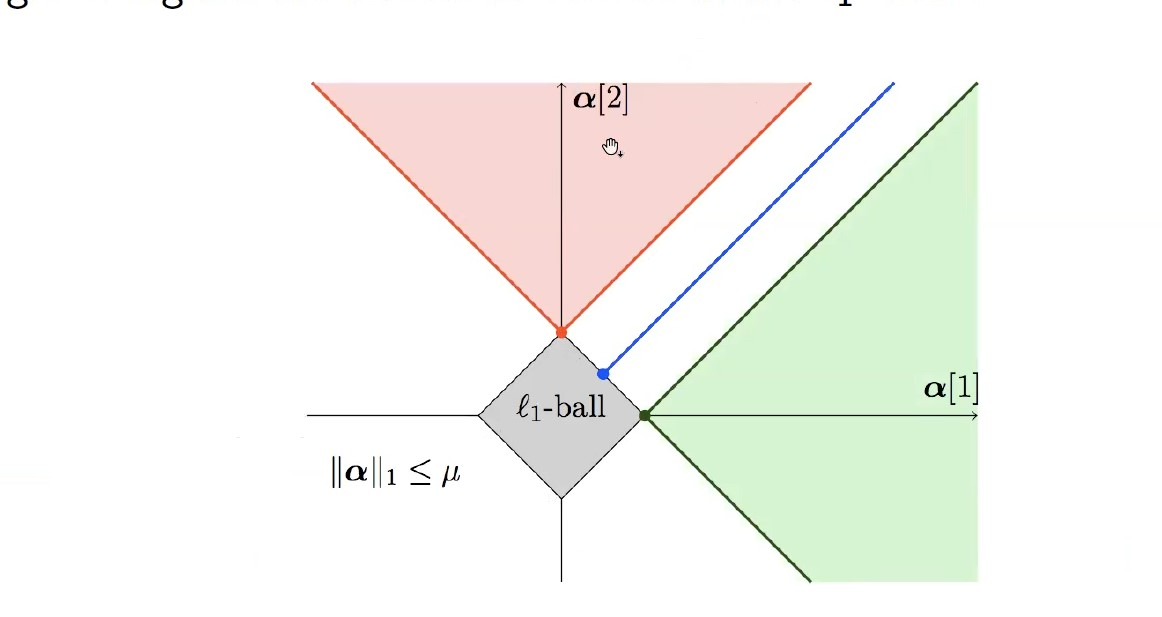
\includegraphics[width=10cm]{lecture_notes/lecture_3/immages/l3_8.jpg} note that the closest point within the constrained area (gray) for any points in the yellow or green area are the points at the axis. 
    \iitem it is only within that white area, where a non-corner solution is closer, and thus don't have a sparse solution
    \item this means that the $\ell_{1}$ favors  solutions that are on the coroner more than others
\end{itemize}
\subsection{optimization perspective}
\item for $\ell_{2}$ regularization 
\begin{itemize}
    \item as $w_i$ becomes smaller there is less and less penalty. like if $w_i\leq 1$ then $|w_i|_2=w_i^2\leq 1$ and specifically points that are very small have almost no penalty
    \item the gradient which determines the direction of optimization see's that as $w_i$ approaches 0 $||w_i||_{2}$ gets smaller, so in trying to minimize $f(X)+\lambda||w||_{2}$ it makes more sense to focus on points with a larger magnitude instead of send $w_i$ all the way to zero
    \item so that is there is less incentive to make a small weight equal to exactly zero
\end{itemize}
\item what for $\ell_{1}$
\begin{itemize}
    \item $||w||_{1}=|w|$ so the gradient will stay the same as $w_i$ goes to zero 
    \item so the gradient will always be 1 or -1, even if you are very close to zero it makes sense to set the weights to exactly zero instead of having them be very small but non-zero
\end{itemize}
\subsection{ l q norm}
\item we can generalize the norm to the  the l q norm $\ell_{q}:||w||_{q}^{q}=|w_1|^{q}+|w_2|^{1}+...+|w_n|^{q}$
\item 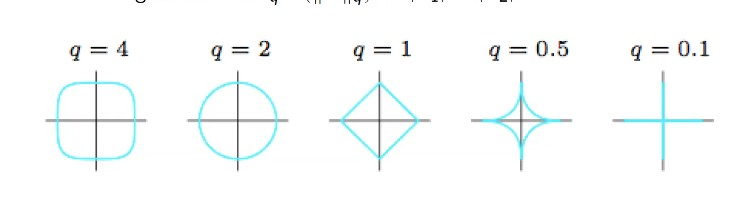
\includegraphics[width=10cm]{lecture_notes/lecture_3/immages/l3_10.jpg}
\item note that $q$ is only really defined as a norm for $q\geq 1$ because other Wise the triangle inequality might fail
\item q gets larger approaches a square
\item q goes to zero, means that we only allow things to happen on the axis. 
\item also when $q<1$ then $\ell_{Q}$ is non convex but hard to optimize
\item $\ell_{0}$ is the number of non-zero weights but is very hard to optimize
\section{minimizing the lasso objective}
\item the ridge objective is differentiable  
\item the lasso objective function $$min_{w\in \mathbb{R}^{d}\Sigma_i=1}^{n}(w^{t}x_i-y_i)^{2}+\lambda||w||_{1}$$
\item notice that the $\ell_{1}$ norm is non differentiable
\item there are three approaches for finding the min
\begin{itemize}
    \item quadratic programming g
    \item projected SGD
    \item coordinate descent 
\end{itemize}
\subsection{quadratic programming }
\itemt consider any number $a\in \mathbb{R}$
\item call the positive part of a $$a^{+}=a1(a\geq 0)$$
\item call the negative part of a $$a^{-}=a1(a\leq 0)$$
\item is it always the case that $a^{+}\geq 0$ and $a^{-}\leq 0$ yes clearly
\item how do we write $a $ in terms of $a^{+},a^{-}$? as $a^{+}-a^{-}$ 
\item how do we write $|a|$ in terms of $a^{+}, a^{-}$ $|a|=w^{+}+w^{-}$
\item using this we can rewrite the objective function of the lasso regression problem as 
$$min_{w^{+},w^{-}}\Sigma_{i=}1^{n}((w^+-w^-)^{T}x_i-y_i)^{2}+\lambda (w^{+}+w^{-}) \text{s.t} w^{+}, w^{-}\geq 0 \forall i$$
\item using this the objective function is both convex and differentiable?
\item this objective function has two variables,  so we can use an quadratic problem solver
\item this quadratic problem solver just sees two variables and two constraints it does not now that $w_{i}^{+}$ and $w_{i}^{-}$ to be the positive and negative part of $w_i$
\item turns of these conditions will be satisfied any way 
\item we do not need the constraint that $a+b=|w|$
\subsection{proof}
\item the goal is to show that $$min_{W}min_{a,b}\Sigma_{i=1}^{n}((a-b)^t x_i-y_i)^{2}+\lambda 1^{t})(a+b) \text{subject to }a_i\geq 0 \forall i, b_i\geq 0 \forall i , a-b=2, a+b=|W|$$
\item  we don't need $a+b=|W|$
\item suppose we have $min(a^{*}, b^{*})=0$ 
\item i think the BASIC logic here is is already set that $a-b$=w thus$\Sigma_{i=1}^{n}((a-b)^t x_i-y_i)^{2}$ this part will not change 
\item on the other hand, if we do not have that constraint we are going to want to minimize $\lambda (a+b)$ that can best be archived by one of the two being set to zero so we do not really need the constraint. 
\subsection{proof II}
\item given our objective function  is \item the goal is to show that $$min_{W}min_{a,b}\Sigma_{i=1}^{n}((a-b)^t x_i-y_i)^{2}+\lambda 1^{t})(a+b) \text{subject to }a_i\geq 0 \forall i, b_i\geq 0 \forall i , a-b=w,$$
\item we can remove the $min_{w}$ and the constraint $a-b=w$
\item we can switch the order of minimization and write this problem as $$min_{a,b}min_{w}\Sigma_{i=1}^{n}((a-b)^t x_i-y_i)^{2}+\lambda 1^{t})(a+b) \text{subject to }a_i\geq 0 \forall i, b_i\geq 0 \forall i , a-b=w,$$ i mean first off it is clear that the a-b=w so minimizing one is the same as minimizing the other 
\item then it does not matter if a-b=w, our goal is to minimize the function with min a-b so naturally that will hold 
\item so in other words we can just write the objective as $$min_{a,b}\Sigma_{i=1}^{n}((a-b)^t x_i-y_i)^{2}+\lambda 1^{t}(a+b) \text{subject to }a_i\geq 0 \forall i, b_i\geq 0 \forall i$$
\subsection{projected SGD}
\item SGD is stochastic gradient descent 
\item now that we have a differentiable objective we can use gradient descent 
\item we can handle the constraints using projected SGD, in which after each step we project the variables back onto our constrained 
\item in other words
\begin{itemize}
    \item we project $w^{+},w^{-}$ into the constraint set 
    \item that is if any component of $w^{+}$ or $w^{-}$ becomes negative we set it back to zero
\end{itemize}
\subsection{coordinate gradient descent}
\item our goal is to minimize $L(w)=L(w_1...w_d)$ over $(w_1,...w_d)\in \mathbb{R}^{d} $
\item in gradient descent or SGD each step potentially changes all entries of w
\item in coordinate descent each step adjust only a single coordinate $w_i$ that is $w_i^{new}=argmin_{w_i}L(w_1,....w_{i-1},w_{i},w_{i+1}...w_{d})$
\item solving the argmin of a particular coordinate may itself be an iterative process 
\tiem coordinate descent is an effective method when it is easier to minimize with respect to one coordinate at a time instead of all of them 
\item algorithm 
\begin{itemize}
    \item goal is to minimize $L(w)=L(w_1...w_d)$ over $(w_1..w_d)\in\mathbb{R}^{d}$
    \item we initialize w=0
    \item while not converged
    \begin{itemize}
        \item chose a coordinate $j\in \{1...d\}$
        \item $w_{j}^{new}\leftarrow argmin_{wj}L(w_1^{t}....w_{j-1}^{t}, w_{J} , w_{j-1}^{t}...w_{d}^{t})$ that is we minimize with respect to just j
        \item $w_{j}^{t+1}\leftarrow w_{j}^{new}$ and $w^{t+1}\leftarrow w^{t}$
        \item t\leftarrow t+1
    \end{itemize}
\end{itemize}
\item we re randomly chose coordinate j then that is stochastic coordinate descent 
\item it we cycle through choices of coordinated j then that is cyclical coordinate descent 

\subsection{coordinate descent methods for lasso}
\item so this one coordinate  weight at a time has an analytical solution $\hat{w}_{j}=argmin_{w_{j}\in \mathbb{R}}\Sigma_{i=1}^{n}(w^{t}x_i-y_i)^2+\lambda |w|_{1}$ 
\item 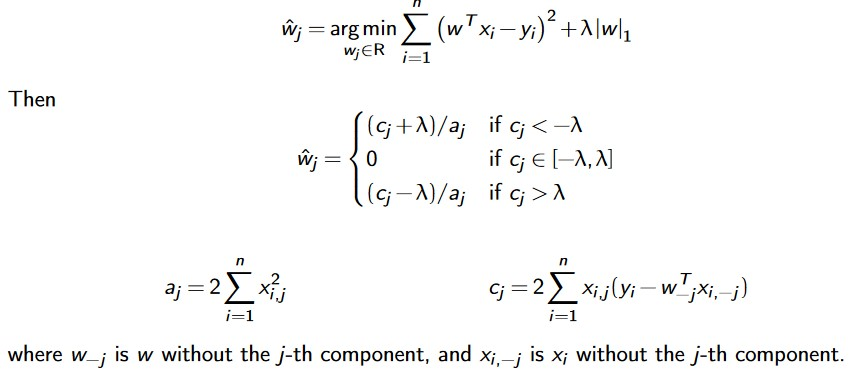
\includegraphics[width =10cm]{lecture_notes/lecture_3/immages/l3_11.jpg}
\subsection{coordinate descent in general}
\item in general coordinate descent is not comparative with gradient descent since its rate of convergence is slower while its computational cost per iteration is similar 
\item it however works really well for certain problems 
\item and it is very simple and easy to implement 
\item it works well for lasso regression and SVMs

\end{itemize}
\end{document}
